\chapter{Graded modalities}



\section{Conditionals}

\section{Quantum and relation with symmetric subspaces and construction of graded modalities}

\section{Discriminating Two Pure Quantum States}
\todo[inline,size=\normalsize]{pôr introdução a quantum state discrimination e a sua importância e de onde vem a melhor estragegia -> livro Barret}



Given a pure $d$-dimensional state \ket{\psi} known to be either \ket{\psi_0} or \ket{\psi_1}, one must guess which state \ket{\psi} is. In quantum state discrimination, we wish to design a measurement to distinguish optimally between \ket{\psi_0} or \ket{\psi_1}. 

Assume with out loss of generality the angle between \ket{\psi_0}  and \ket{\psi_1}, designated $\alpha$, is between $0$ and $\frac{pi}{2}$. Otherwise, replace \ket{\psi_0} is replaced by $- \ket{\psi_0}$.

In this case the best strategy is is to do the projective measurement with \{\ket{v_0}, \ket{v_1}\}, where \ket{v_0}, \ket{v_1}\ are in the span of \ket{\psi_0}  and \ket{\psi_1} such that $\langle v_{0}| v_{0} \rangle = 0$, they are symmetric with
respect to the angle bisector of \ket{\psi_0}  and \ket{\psi_1}, and \ket{v_i} is closer to  \ket{\psi_i} for $i = 0, 1$. On outcome $“i”$, we guess $\psi_i$.

\begin{figure} [H] 
    \centering
    \begin{center}
        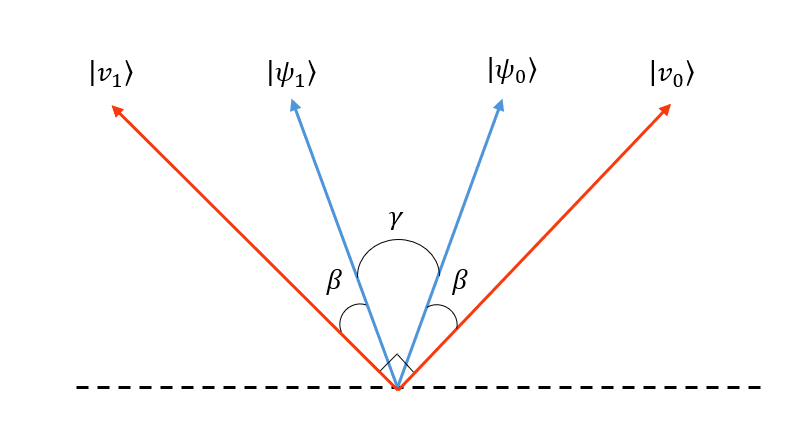
\includegraphics[width=0.6\textwidth]{images/qsd_0.png}
    \end{center}
\caption{Optimal minimum error measurement for discriminating between the pure states \ket{\psi_0}  and  \ket{\psi_1}. This is a
projective measurement onto the states \ket{v_0}  and  \ket{v_1}, symmetrically located on either side of the signal states and shown in red here. $\gamma$ is  the angle between the states \ket{\psi_0}  and  \ket{\psi_1}. $\beta$ is the angle between the states \ket{\psi_0}  and  \ket{v_0} \big/ \ket{\psi_1}  and  \ket{v_1} .}
\label{fig:qsd}
\end{figure}

The probability of success using the best strategy is

\begin{equation*}
    P_{succ} = \langle \psi_{0}| v_{0} \rangle = \cos^2(\beta) = \cos^2 \left(\frac{\pi/2 - \gamma}{2}\right) = \frac{1}{2} + \frac{1}{2} \cos(\pi/2 -\gamma) = \frac{1}{2} + \frac{1}{2} \sin(\gamma)
\end{equation*}

\subsection{QSD for two pure states: quantum lambda calculus formulation}

Since the quantum lambda calculus presented allows only for explicit projective measurements in the computational basis, it is necessary to rotate the state \ket{\psi} so that \ket{v_0} and \ket{v_1} coincide with the computational basis. This can be done by applying a unitary $U$ to the state \ket{\psi} such that $U \ket{v_0} = \ket{0}$. 

Observing \autoref{fig:qsd} is possible to conclude that $\beta =  \frac{\frac{\pi}{2}-\gamma}{2} = \frac{\pi}{4} - \frac{\gamma}{2}$. Therefore,

\begin{equation}
    \begin{split}
        \ket{v_0} =R^{\dag}_{\beta} \ket{\psi_0} & = \begin{pmatrix}
        \cos{ \left(\frac{\pi}{4} - \frac{\gamma}{2}\right)}  & \sin{ \left(\frac{\pi}{4} - \frac{\gamma}{2}\right)} \\
       - \sin{ \left(\frac{\pi}{4} - \frac{\gamma}{2}\right)}  &  \cos{ \left(\frac{\pi}{4} - \frac{\gamma}{2}\right)} \end{pmatrix} \begin{pmatrix}
        \cos{ \left(\frac{\theta}{2}\right)}   \\
       e^{i \phi}\sin{ \left(\frac{\theta}{2}\right)}  \end{pmatrix} \\
       & = \begin{pmatrix}
        \cos{ \left(\frac{\pi}{4} - \frac{\gamma}{2}\right)}  \cos{ \left(\frac{\theta}{2}\right)}  + \sin{ \left(\frac{\pi}{4} - \frac{\gamma}{2}\right)} e^{i \phi}\sin{ \left(\frac{\theta}{2}\right)}  \\
       - \sin{ \left(\frac{\pi}{4} - \frac{\gamma}{2}\right)}  \cos{ \left(\frac{\theta}{2}\right)}  +  \cos{ \left(\frac{\pi}{4} - \frac{\gamma}{2}\right)} e^{i \phi}\sin{ \left(\frac{\theta}{2}\right)}   \end{pmatrix} 
    \end{split}
\end{equation}

Consequently, 

\begin{equation}
    \begin{split}
        \ket{v_1}  = \begin{pmatrix}
         \sin{ \left(\frac{\pi}{4} - \frac{\gamma}{2}\right)}  \cos{ \left(\frac{\theta}{2}\right)}  -  \cos{ \left(\frac{\pi}{4} - \frac{\gamma}{2}\right)} e^{i \phi}\sin{ \left(\frac{\theta}{2}\right)}   
        \\
        \cos{ \left(\frac{\pi}{4} - \frac{\gamma}{2}\right)}  \cos{ \left(\frac{\theta}{2}\right)}  + \sin{ \left(\frac{\pi}{4} - \frac{\gamma}{2}\right)} e^{i \phi}\sin{ \left(\frac{\theta}{2}\right)}  \end{pmatrix} 
    \end{split}
\end{equation}

As a result,
\begin{equation}
    \begin{split}
        U =  \begin{pmatrix} \cos{ \left(\frac{\pi}{4} - \frac{\gamma}{2}\right)}  \cos{ \left(\frac{\theta}{2}\right)}  + \sin{ \left(\frac{\pi}{4} - \frac{\gamma}{2}\right)} e^{-i \phi}\sin{ \left(\frac{\theta}{2}\right)}  & - \sin{ \left(\frac{\pi}{4} - \frac{\gamma}{2}\right)}  \cos{ \left(\frac{\theta}{2}\right)}  +  \cos{ \left(\frac{\pi}{4} - \frac{\gamma}{2}\right)} e^{-i \phi}\sin{ \left(\frac{\theta}{2}\right)}   \\
            \sin{ \left(\frac{\pi}{4} - \frac{\gamma}{2}\right)}  \cos{ \left(\frac{\theta}{2}\right)}  -  \cos{ \left(\frac{\pi}{4} - \frac{\gamma}{2}\right)} e^{-i \phi}\sin{ \left(\frac{\theta}{2}\right)}  &  \cos{ \left(\frac{\pi}{4} - \frac{\gamma}{2}\right)}  \cos{ \left(\frac{\theta}{2}\right)}  + \sin{ \left(\frac{\pi}{4} - \frac{\gamma}{2}\right)} e^{-i \phi}\sin{ \left(\frac{\theta}{2}\right)}  \end{pmatrix} 
    \end{split}
\end{equation}

When $\ket{\psi} = \ket{\psi_0}$, one has that,
\begin{equation}
    \begin{split}
        &U \ket{\psi} = \\
        &\scriptsize{
            \begin{pmatrix} 
                \left[\cos{ \left(\frac{\pi}{4} - \frac{\gamma}{2}\right)}  \cos{ \left(\frac{\theta}{2}\right)}  + \sin{ \left(\frac{\pi}{4} - \frac{\gamma}{2}\right)} e^{-i \phi}\sin{ \left(\frac{\theta}{2}\right)}\right] \cos{ \left(\frac{\theta}{2}\right)}  +  
                \left[ - \sin{ \left(\frac{\pi}{4} - \frac{\gamma}{2}\right)}  \cos{ \left(\frac{\theta}{2}\right)}  +  \cos{ \left(\frac{\pi}{4} - \frac{\gamma}{2}\right)} e^{-i \phi}\sin{ \left(\frac{\theta}{2}\right)} \right] e^{i \phi}\sin{ \left(\frac{\theta}{2}\right)} \\
                \left[\sin{ \left(\frac{\pi}{4} - \frac{\gamma}{2}\right)}  \cos{ \left(\frac{\theta}{2}\right)}  -  \cos{ \left(\frac{\pi}{4} - \frac{\gamma}{2}\right)} e^{-i \phi}\sin{ \left(\frac{\theta}{2}\right)}\right]\cos{ \left(\frac{\theta}{2}\right)} + \left[ \cos{ \left(\frac{\pi}{4} - \frac{\gamma}{2}\right)}  \cos{ \left(\frac{\theta}{2}\right)}  + \sin{ \left(\frac{\pi}{4} - \frac{\gamma}{2}\right)} e^{-i \phi}\sin{ \left(\frac{\theta}{2}\right)} \right] e^{i \phi}\sin{ \left(\frac{\theta}{2}\right)}
            \end{pmatrix}  } \\
        & = \begin{pmatrix} \cos{ \left(\frac{\pi}{4} - \frac{\gamma}{2}\right)} \frac{\cos{ \left(\theta\right)}+1} {2}   + e^{-i \phi} \sin{ \left(\frac{\pi}{4} - \frac{\gamma}{2}\right)} \frac{\sin{ \left(\theta\right)}} {2} - e^{i \phi} \sin{ \left(\frac{\pi}{4} - \frac{\gamma}{2}\right)} \frac{\sin{ \left(\theta\right)}} {2} +  \cos{ \left(\frac{\pi}{4} - \frac{\gamma}{2}\right)} \frac{\cos{ 1- \left(\theta\right)}} {2} \\
        \sin{ \left(\frac{\pi}{4} - \frac{\gamma}{2}\right)} \frac{\cos{ \left(\theta\right)}+1} {2}   - e^{-i \phi} \cos{ \left(\frac{\pi}{4} - \frac{\gamma}{2}\right)} \frac{\sin{ \left(\theta\right)}} {2} + e^{i \phi} \cos{ \left(\frac{\pi}{4} - \frac{\gamma}{2}\right)} \frac{\sin{ \left(\theta\right)}} {2} +  \sin{ \left(\frac{\pi}{4} - \frac{\gamma}{2}\right)} \frac{\cos{ 1- \left(\theta\right)}} {2}  
            \end{pmatrix} \\
            & = \begin{pmatrix} \cos{ \left(\frac{\pi}{4} - \frac{\gamma}{2}\right)}   + (e^{-i \phi}-e^{i \phi}) \sin{ \left(\frac{\pi}{4} - \frac{\gamma}{2}\right)} \frac{\sin{ \left(\theta\right)}} {2} \\
            \sin{ \left(\frac{\pi}{4} - \frac{\gamma}{2}\right)} \  (- e^{-i \phi} + e^{i \phi} ) \cos{ \left(\frac{\pi}{4} - \frac{\gamma}{2}\right)} \frac{\sin{ \left(\theta\right)}} {2} \end{pmatrix} \\
            & = \begin{pmatrix} \cos{ \left(\frac{\pi}{4} - \frac{\gamma}{2}\right)}   + 2i \sin{(\phi)} (\cos{ \left(\frac{\pi}{4} - \frac{\gamma}{2}-\theta\right)} - \cos{ \left(\frac{\pi}{4} - \frac{\gamma}{2}+\theta \right)} )\\
            \sin{ \left(\frac{\pi}{4} - \frac{\gamma}{2}\right)} \  - 2i \sin{(\phi)} (\sin{ \left(\frac{\pi}{4} - \frac{\gamma}{2}+\theta\right)} - \sin{ \left(\frac{\pi}{4} - \frac{\gamma}{2}-\theta \right)} ) \end{pmatrix} 
    \end{split}
\end{equation}

%Given the direction of the rotation, the angle $\alpha$ is negative, so the rotation is $R_{-\alpha}$ which also correspons to $R^{\dag}_{\alpha}$.

%As a result, the quantum discrimination for two pure states can be formulated as follows:
%\begin{align*}
  %q: \textit{qbit}\hspace{3 pt} \triangleright \hspace{3 pt} \textit{meas} (U (q)) 
%\end{align*}

